% Created by tikzDevice version 0.6.2-92-0ad2792 on 2013-03-04 16:57:04
% !TEX encoding = UTF-8 Unicode
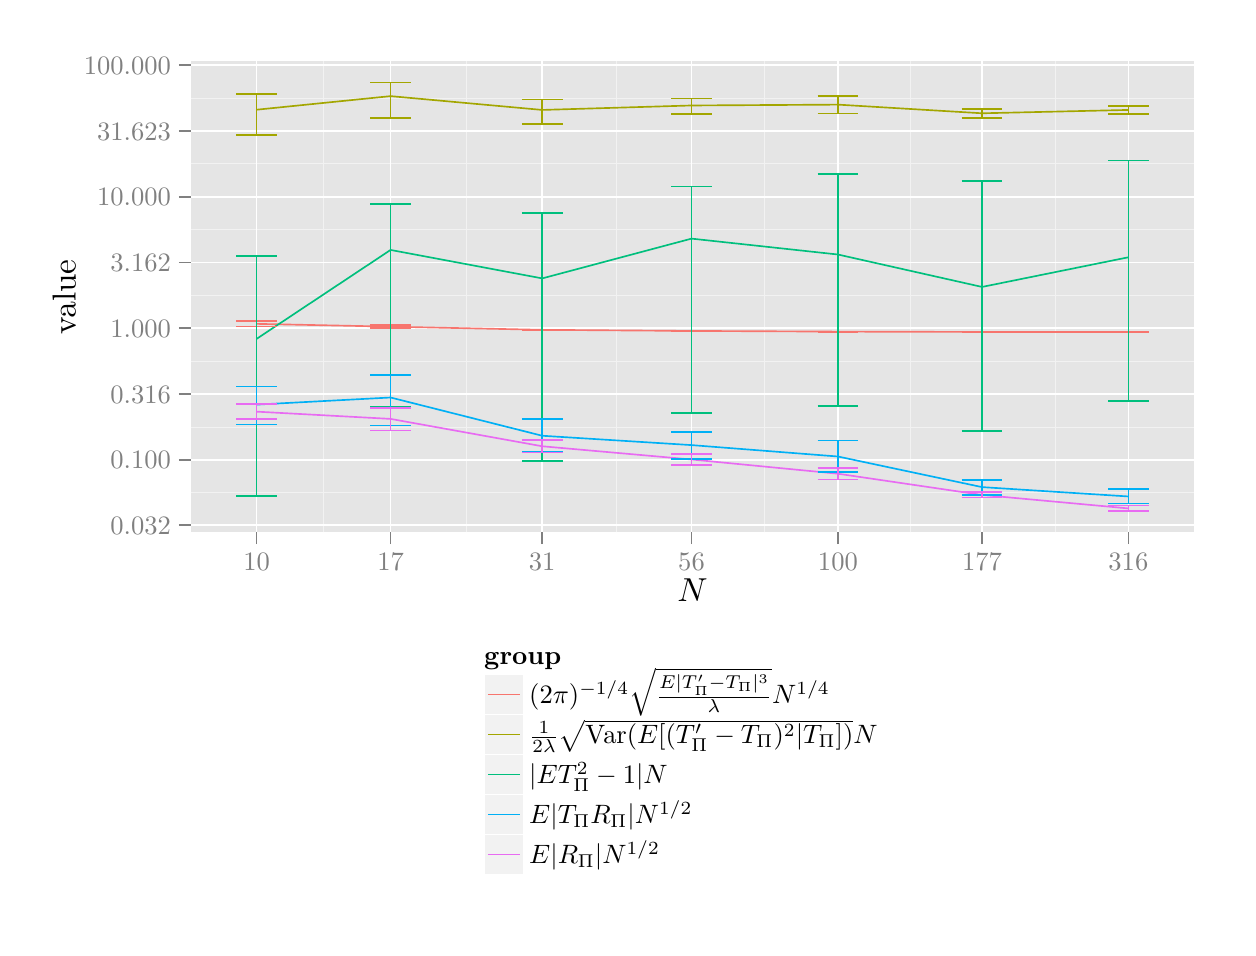
\begin{tikzpicture}[x=1pt,y=1pt]
\definecolor[named]{fillColor}{rgb}{1.00,1.00,1.00}
\path[use as bounding box,fill=fillColor,fill opacity=0.00] (0,0) rectangle (433.62,325.21);
\begin{scope}
\path[clip] (  0.00,  0.00) rectangle (433.62,325.21);
\definecolor[named]{drawColor}{rgb}{1.00,1.00,1.00}
\definecolor[named]{fillColor}{rgb}{1.00,1.00,1.00}

\path[draw=drawColor,line width= 0.6pt,line join=round,line cap=round,fill=fillColor] (  0.00,  0.00) rectangle (433.62,325.21);
\end{scope}
\begin{scope}
\path[clip] ( 58.88,142.81) rectangle (421.57,313.17);
\definecolor[named]{fillColor}{rgb}{0.90,0.90,0.90}

\path[fill=fillColor] ( 58.88,142.81) rectangle (421.57,313.17);
\definecolor[named]{drawColor}{rgb}{0.95,0.95,0.95}

\path[draw=drawColor,line width= 0.3pt,line join=round] ( 58.88,157.30) --
	(421.57,157.30);

\path[draw=drawColor,line width= 0.3pt,line join=round] ( 58.88,180.94) --
	(421.57,180.94);

\path[draw=drawColor,line width= 0.3pt,line join=round] ( 58.88,204.70) --
	(421.57,204.70);

\path[draw=drawColor,line width= 0.3pt,line join=round] ( 58.88,228.47) --
	(421.57,228.47);

\path[draw=drawColor,line width= 0.3pt,line join=round] ( 58.88,252.23) --
	(421.57,252.23);

\path[draw=drawColor,line width= 0.3pt,line join=round] ( 58.88,275.99) --
	(421.57,275.99);

\path[draw=drawColor,line width= 0.3pt,line join=round] ( 58.88,299.75) --
	(421.57,299.75);

\path[draw=drawColor,line width= 0.3pt,line join=round] (106.92,142.81) --
	(106.92,313.17);

\path[draw=drawColor,line width= 0.3pt,line join=round] (158.53,142.81) --
	(158.53,313.17);

\path[draw=drawColor,line width= 0.3pt,line join=round] (212.91,142.81) --
	(212.91,313.17);

\path[draw=drawColor,line width= 0.3pt,line join=round] (266.33,142.81) --
	(266.33,313.17);

\path[draw=drawColor,line width= 0.3pt,line join=round] (318.82,142.81) --
	(318.82,313.17);

\path[draw=drawColor,line width= 0.3pt,line join=round] (371.30,142.81) --
	(371.30,313.17);
\definecolor[named]{drawColor}{rgb}{1.00,1.00,1.00}

\path[draw=drawColor,line width= 0.6pt,line join=round] ( 58.88,145.54) --
	(421.57,145.54);

\path[draw=drawColor,line width= 0.6pt,line join=round] ( 58.88,169.06) --
	(421.57,169.06);

\path[draw=drawColor,line width= 0.6pt,line join=round] ( 58.88,192.81) --
	(421.57,192.81);

\path[draw=drawColor,line width= 0.6pt,line join=round] ( 58.88,216.59) --
	(421.57,216.59);

\path[draw=drawColor,line width= 0.6pt,line join=round] ( 58.88,240.35) --
	(421.57,240.35);

\path[draw=drawColor,line width= 0.6pt,line join=round] ( 58.88,264.11) --
	(421.57,264.11);

\path[draw=drawColor,line width= 0.6pt,line join=round] ( 58.88,287.87) --
	(421.57,287.87);

\path[draw=drawColor,line width= 0.6pt,line join=round] ( 58.88,311.63) --
	(421.57,311.63);

\path[draw=drawColor,line width= 0.6pt,line join=round] ( 82.72,142.81) --
	( 82.72,313.17);

\path[draw=drawColor,line width= 0.6pt,line join=round] (131.13,142.81) --
	(131.13,313.17);

\path[draw=drawColor,line width= 0.6pt,line join=round] (185.93,142.81) --
	(185.93,313.17);

\path[draw=drawColor,line width= 0.6pt,line join=round] (239.88,142.81) --
	(239.88,313.17);

\path[draw=drawColor,line width= 0.6pt,line join=round] (292.78,142.81) --
	(292.78,313.17);

\path[draw=drawColor,line width= 0.6pt,line join=round] (344.86,142.81) --
	(344.86,313.17);

\path[draw=drawColor,line width= 0.6pt,line join=round] (397.74,142.81) --
	(397.74,313.17);
\definecolor[named]{drawColor}{rgb}{0.97,0.46,0.43}

\path[draw=drawColor,line width= 0.6pt,line join=round] ( 82.72,218.18) --
	(131.13,217.17) --
	(185.93,216.02) --
	(239.88,215.62) --
	(292.78,215.38) --
	(344.86,215.26) --
	(397.74,215.21);
\definecolor[named]{drawColor}{rgb}{0.64,0.65,0.00}

\path[draw=drawColor,line width= 0.6pt,line join=round] ( 82.72,295.56) --
	(131.13,300.47) --
	(185.93,295.48) --
	(239.88,297.09) --
	(292.78,297.40) --
	(344.86,294.27) --
	(397.74,295.48);
\definecolor[named]{drawColor}{rgb}{0.00,0.75,0.49}

\path[draw=drawColor,line width= 0.6pt,line join=round] ( 82.72,212.76) --
	(131.13,244.89) --
	(185.93,234.61) --
	(239.88,248.98) --
	(292.78,243.24) --
	(344.86,231.52) --
	(397.74,242.24);
\definecolor[named]{drawColor}{rgb}{0.00,0.69,0.96}

\path[draw=drawColor,line width= 0.6pt,line join=round] ( 82.72,189.00) --
	(131.13,191.57) --
	(185.93,177.75) --
	(239.88,174.37) --
	(292.78,170.25) --
	(344.86,159.19) --
	(397.74,155.81);
\definecolor[named]{drawColor}{rgb}{0.91,0.42,0.95}

\path[draw=drawColor,line width= 0.6pt,line join=round] ( 82.72,186.46) --
	(131.13,183.84) --
	(185.93,173.95) --
	(239.88,169.17) --
	(292.78,164.03) --
	(344.86,156.36) --
	(397.74,151.49);
\definecolor[named]{drawColor}{rgb}{0.97,0.46,0.43}

\path[draw=drawColor,line width= 0.6pt,line join=round] ( 75.37,219.15) --
	( 90.07,219.15);

\path[draw=drawColor,line width= 0.6pt,line join=round] ( 82.72,219.15) --
	( 82.72,217.20);

\path[draw=drawColor,line width= 0.6pt,line join=round] ( 75.37,217.20) --
	( 90.07,217.20);

\path[draw=drawColor,line width= 0.6pt,line join=round] (123.78,217.78) --
	(138.48,217.78);

\path[draw=drawColor,line width= 0.6pt,line join=round] (131.13,217.78) --
	(131.13,216.61);

\path[draw=drawColor,line width= 0.6pt,line join=round] (123.78,216.61) --
	(138.48,216.61);

\path[draw=drawColor,line width= 0.6pt,line join=round] (178.58,216.20) --
	(193.28,216.20);

\path[draw=drawColor,line width= 0.6pt,line join=round] (185.93,216.20) --
	(185.93,215.85);

\path[draw=drawColor,line width= 0.6pt,line join=round] (178.58,215.85) --
	(193.28,215.85);

\path[draw=drawColor,line width= 0.6pt,line join=round] (232.53,215.69) --
	(247.23,215.69);

\path[draw=drawColor,line width= 0.6pt,line join=round] (239.88,215.69) --
	(239.88,215.54);

\path[draw=drawColor,line width= 0.6pt,line join=round] (232.53,215.54) --
	(247.23,215.54);

\path[draw=drawColor,line width= 0.6pt,line join=round] (285.42,215.42) --
	(300.13,215.42);

\path[draw=drawColor,line width= 0.6pt,line join=round] (292.78,215.42) --
	(292.78,215.35);

\path[draw=drawColor,line width= 0.6pt,line join=round] (285.42,215.35) --
	(300.13,215.35);

\path[draw=drawColor,line width= 0.6pt,line join=round] (337.51,215.28) --
	(352.22,215.28);

\path[draw=drawColor,line width= 0.6pt,line join=round] (344.86,215.28) --
	(344.86,215.25);

\path[draw=drawColor,line width= 0.6pt,line join=round] (337.51,215.25) --
	(352.22,215.25);

\path[draw=drawColor,line width= 0.6pt,line join=round] (390.39,215.21) --
	(405.09,215.21);

\path[draw=drawColor,line width= 0.6pt,line join=round] (397.74,215.21) --
	(397.74,215.20);

\path[draw=drawColor,line width= 0.6pt,line join=round] (390.39,215.20) --
	(405.09,215.20);
\definecolor[named]{drawColor}{rgb}{0.64,0.65,0.00}

\path[draw=drawColor,line width= 0.6pt,line join=round] ( 75.37,301.27) --
	( 90.07,301.27);

\path[draw=drawColor,line width= 0.6pt,line join=round] ( 82.72,301.27) --
	( 82.72,286.33);

\path[draw=drawColor,line width= 0.6pt,line join=round] ( 75.37,286.33) --
	( 90.07,286.33);

\path[draw=drawColor,line width= 0.6pt,line join=round] (123.78,305.43) --
	(138.48,305.43);

\path[draw=drawColor,line width= 0.6pt,line join=round] (131.13,305.43) --
	(131.13,292.48);

\path[draw=drawColor,line width= 0.6pt,line join=round] (123.78,292.48) --
	(138.48,292.48);

\path[draw=drawColor,line width= 0.6pt,line join=round] (178.58,299.20) --
	(193.28,299.20);

\path[draw=drawColor,line width= 0.6pt,line join=round] (185.93,299.20) --
	(185.93,290.45);

\path[draw=drawColor,line width= 0.6pt,line join=round] (178.58,290.45) --
	(193.28,290.45);

\path[draw=drawColor,line width= 0.6pt,line join=round] (232.53,299.59) --
	(247.23,299.59);

\path[draw=drawColor,line width= 0.6pt,line join=round] (239.88,299.59) --
	(239.88,294.04);

\path[draw=drawColor,line width= 0.6pt,line join=round] (232.53,294.04) --
	(247.23,294.04);

\path[draw=drawColor,line width= 0.6pt,line join=round] (285.42,300.58) --
	(300.13,300.58);

\path[draw=drawColor,line width= 0.6pt,line join=round] (292.78,300.58) --
	(292.78,294.25);

\path[draw=drawColor,line width= 0.6pt,line join=round] (285.42,294.25) --
	(300.13,294.25);

\path[draw=drawColor,line width= 0.6pt,line join=round] (337.51,295.82) --
	(352.22,295.82);

\path[draw=drawColor,line width= 0.6pt,line join=round] (344.86,295.82) --
	(344.86,292.62);

\path[draw=drawColor,line width= 0.6pt,line join=round] (337.51,292.62) --
	(352.22,292.62);

\path[draw=drawColor,line width= 0.6pt,line join=round] (390.39,296.95) --
	(405.09,296.95);

\path[draw=drawColor,line width= 0.6pt,line join=round] (397.74,296.95) --
	(397.74,294.01);

\path[draw=drawColor,line width= 0.6pt,line join=round] (390.39,294.01) --
	(405.09,294.01);
\definecolor[named]{drawColor}{rgb}{0.00,0.75,0.49}

\path[draw=drawColor,line width= 0.6pt,line join=round] ( 75.37,242.69) --
	( 90.07,242.69);

\path[draw=drawColor,line width= 0.6pt,line join=round] ( 82.72,242.69) --
	( 82.72,155.96);

\path[draw=drawColor,line width= 0.6pt,line join=round] ( 75.37,155.96) --
	( 90.07,155.96);

\path[draw=drawColor,line width= 0.6pt,line join=round] (123.78,261.59) --
	(138.48,261.59);

\path[draw=drawColor,line width= 0.6pt,line join=round] (131.13,261.59) --
	(131.13,188.25);

\path[draw=drawColor,line width= 0.6pt,line join=round] (123.78,188.25) --
	(138.48,188.25);

\path[draw=drawColor,line width= 0.6pt,line join=round] (178.58,258.35) --
	(193.28,258.35);

\path[draw=drawColor,line width= 0.6pt,line join=round] (185.93,258.35) --
	(185.93,168.70);

\path[draw=drawColor,line width= 0.6pt,line join=round] (178.58,168.70) --
	(193.28,168.70);

\path[draw=drawColor,line width= 0.6pt,line join=round] (232.53,267.84) --
	(247.23,267.84);

\path[draw=drawColor,line width= 0.6pt,line join=round] (239.88,267.84) --
	(239.88,185.89);

\path[draw=drawColor,line width= 0.6pt,line join=round] (232.53,185.89) --
	(247.23,185.89);

\path[draw=drawColor,line width= 0.6pt,line join=round] (285.42,272.41) --
	(300.13,272.41);

\path[draw=drawColor,line width= 0.6pt,line join=round] (292.78,272.41) --
	(292.78,188.49);

\path[draw=drawColor,line width= 0.6pt,line join=round] (285.42,188.49) --
	(300.13,188.49);

\path[draw=drawColor,line width= 0.6pt,line join=round] (337.51,269.78) --
	(352.22,269.78);

\path[draw=drawColor,line width= 0.6pt,line join=round] (344.86,269.78) --
	(344.86,179.51);

\path[draw=drawColor,line width= 0.6pt,line join=round] (337.51,179.51) --
	(352.22,179.51);

\path[draw=drawColor,line width= 0.6pt,line join=round] (390.39,277.16) --
	(405.09,277.16);

\path[draw=drawColor,line width= 0.6pt,line join=round] (397.74,277.16) --
	(397.74,190.37);

\path[draw=drawColor,line width= 0.6pt,line join=round] (390.39,190.37) --
	(405.09,190.37);
\definecolor[named]{drawColor}{rgb}{0.00,0.69,0.96}

\path[draw=drawColor,line width= 0.6pt,line join=round] ( 75.37,195.60) --
	( 90.07,195.60);

\path[draw=drawColor,line width= 0.6pt,line join=round] ( 82.72,195.60) --
	( 82.72,181.85);

\path[draw=drawColor,line width= 0.6pt,line join=round] ( 75.37,181.85) --
	( 90.07,181.85);

\path[draw=drawColor,line width= 0.6pt,line join=round] (123.78,199.78) --
	(138.48,199.78);

\path[draw=drawColor,line width= 0.6pt,line join=round] (131.13,199.78) --
	(131.13,181.44);

\path[draw=drawColor,line width= 0.6pt,line join=round] (123.78,181.44) --
	(138.48,181.44);

\path[draw=drawColor,line width= 0.6pt,line join=round] (178.58,183.82) --
	(193.28,183.82);

\path[draw=drawColor,line width= 0.6pt,line join=round] (185.93,183.82) --
	(185.93,172.06);

\path[draw=drawColor,line width= 0.6pt,line join=round] (178.58,172.06) --
	(193.28,172.06);

\path[draw=drawColor,line width= 0.6pt,line join=round] (232.53,179.04) --
	(247.23,179.04);

\path[draw=drawColor,line width= 0.6pt,line join=round] (239.88,179.04) --
	(239.88,169.39);

\path[draw=drawColor,line width= 0.6pt,line join=round] (232.53,169.39) --
	(247.23,169.39);

\path[draw=drawColor,line width= 0.6pt,line join=round] (285.42,176.09) --
	(300.13,176.09);

\path[draw=drawColor,line width= 0.6pt,line join=round] (292.78,176.09) --
	(292.78,164.54);

\path[draw=drawColor,line width= 0.6pt,line join=round] (285.42,164.54) --
	(300.13,164.54);

\path[draw=drawColor,line width= 0.6pt,line join=round] (337.51,161.71) --
	(352.22,161.71);

\path[draw=drawColor,line width= 0.6pt,line join=round] (344.86,161.71) --
	(344.86,156.45);

\path[draw=drawColor,line width= 0.6pt,line join=round] (337.51,156.45) --
	(352.22,156.45);

\path[draw=drawColor,line width= 0.6pt,line join=round] (390.39,158.40) --
	(405.09,158.40);

\path[draw=drawColor,line width= 0.6pt,line join=round] (397.74,158.40) --
	(397.74,153.23);

\path[draw=drawColor,line width= 0.6pt,line join=round] (390.39,153.23) --
	(405.09,153.23);
\definecolor[named]{drawColor}{rgb}{0.91,0.42,0.95}

\path[draw=drawColor,line width= 0.6pt,line join=round] ( 75.37,189.31) --
	( 90.07,189.31);

\path[draw=drawColor,line width= 0.6pt,line join=round] ( 82.72,189.31) --
	( 82.72,183.85);

\path[draw=drawColor,line width= 0.6pt,line join=round] ( 75.37,183.85) --
	( 90.07,183.85);

\path[draw=drawColor,line width= 0.6pt,line join=round] (123.78,187.76) --
	(138.48,187.76);

\path[draw=drawColor,line width= 0.6pt,line join=round] (131.13,187.76) --
	(131.13,179.70);

\path[draw=drawColor,line width= 0.6pt,line join=round] (123.78,179.70) --
	(138.48,179.70);

\path[draw=drawColor,line width= 0.6pt,line join=round] (178.58,176.31) --
	(193.28,176.31);

\path[draw=drawColor,line width= 0.6pt,line join=round] (185.93,176.31) --
	(185.93,171.70);

\path[draw=drawColor,line width= 0.6pt,line join=round] (178.58,171.70) --
	(193.28,171.70);

\path[draw=drawColor,line width= 0.6pt,line join=round] (232.53,171.27) --
	(247.23,171.27);

\path[draw=drawColor,line width= 0.6pt,line join=round] (239.88,171.27) --
	(239.88,167.20);

\path[draw=drawColor,line width= 0.6pt,line join=round] (232.53,167.20) --
	(247.23,167.20);

\path[draw=drawColor,line width= 0.6pt,line join=round] (285.42,166.15) --
	(300.13,166.15);

\path[draw=drawColor,line width= 0.6pt,line join=round] (292.78,166.15) --
	(292.78,161.96);

\path[draw=drawColor,line width= 0.6pt,line join=round] (285.42,161.96) --
	(300.13,161.96);

\path[draw=drawColor,line width= 0.6pt,line join=round] (337.51,157.34) --
	(352.22,157.34);

\path[draw=drawColor,line width= 0.6pt,line join=round] (344.86,157.34) --
	(344.86,155.41);

\path[draw=drawColor,line width= 0.6pt,line join=round] (337.51,155.41) --
	(352.22,155.41);

\path[draw=drawColor,line width= 0.6pt,line join=round] (390.39,152.52) --
	(405.09,152.52);

\path[draw=drawColor,line width= 0.6pt,line join=round] (397.74,152.52) --
	(397.74,150.56);

\path[draw=drawColor,line width= 0.6pt,line join=round] (390.39,150.56) --
	(405.09,150.56);
\end{scope}
\begin{scope}
\path[clip] (  0.00,  0.00) rectangle (433.62,325.21);
\definecolor[named]{drawColor}{rgb}{0.50,0.50,0.50}

\node[text=drawColor,anchor=base east,inner sep=0pt, outer sep=0pt, scale=  0.96] at ( 51.77,142.24) {0.032};

\node[text=drawColor,anchor=base east,inner sep=0pt, outer sep=0pt, scale=  0.96] at ( 51.77,165.76) {0.100};

\node[text=drawColor,anchor=base east,inner sep=0pt, outer sep=0pt, scale=  0.96] at ( 51.77,189.50) {0.316};

\node[text=drawColor,anchor=base east,inner sep=0pt, outer sep=0pt, scale=  0.96] at ( 51.77,213.28) {1.000};

\node[text=drawColor,anchor=base east,inner sep=0pt, outer sep=0pt, scale=  0.96] at ( 51.77,237.04) {3.162};

\node[text=drawColor,anchor=base east,inner sep=0pt, outer sep=0pt, scale=  0.96] at ( 51.77,260.80) {10.000};

\node[text=drawColor,anchor=base east,inner sep=0pt, outer sep=0pt, scale=  0.96] at ( 51.77,284.57) {31.623};

\node[text=drawColor,anchor=base east,inner sep=0pt, outer sep=0pt, scale=  0.96] at ( 51.77,308.33) {100.000};
\end{scope}
\begin{scope}
\path[clip] (  0.00,  0.00) rectangle (433.62,325.21);
\definecolor[named]{drawColor}{rgb}{0.50,0.50,0.50}

\path[draw=drawColor,line width= 0.6pt,line join=round] ( 54.61,145.54) --
	( 58.88,145.54);

\path[draw=drawColor,line width= 0.6pt,line join=round] ( 54.61,169.06) --
	( 58.88,169.06);

\path[draw=drawColor,line width= 0.6pt,line join=round] ( 54.61,192.81) --
	( 58.88,192.81);

\path[draw=drawColor,line width= 0.6pt,line join=round] ( 54.61,216.59) --
	( 58.88,216.59);

\path[draw=drawColor,line width= 0.6pt,line join=round] ( 54.61,240.35) --
	( 58.88,240.35);

\path[draw=drawColor,line width= 0.6pt,line join=round] ( 54.61,264.11) --
	( 58.88,264.11);

\path[draw=drawColor,line width= 0.6pt,line join=round] ( 54.61,287.87) --
	( 58.88,287.87);

\path[draw=drawColor,line width= 0.6pt,line join=round] ( 54.61,311.63) --
	( 58.88,311.63);
\end{scope}
\begin{scope}
\path[clip] (  0.00,  0.00) rectangle (433.62,325.21);
\definecolor[named]{drawColor}{rgb}{0.50,0.50,0.50}

\path[draw=drawColor,line width= 0.6pt,line join=round] ( 82.72,138.55) --
	( 82.72,142.81);

\path[draw=drawColor,line width= 0.6pt,line join=round] (131.13,138.55) --
	(131.13,142.81);

\path[draw=drawColor,line width= 0.6pt,line join=round] (185.93,138.55) --
	(185.93,142.81);

\path[draw=drawColor,line width= 0.6pt,line join=round] (239.88,138.55) --
	(239.88,142.81);

\path[draw=drawColor,line width= 0.6pt,line join=round] (292.78,138.55) --
	(292.78,142.81);

\path[draw=drawColor,line width= 0.6pt,line join=round] (344.86,138.55) --
	(344.86,142.81);

\path[draw=drawColor,line width= 0.6pt,line join=round] (397.74,138.55) --
	(397.74,142.81);
\end{scope}
\begin{scope}
\path[clip] (  0.00,  0.00) rectangle (433.62,325.21);
\definecolor[named]{drawColor}{rgb}{0.50,0.50,0.50}

\node[text=drawColor,anchor=base,inner sep=0pt, outer sep=0pt, scale=  0.96] at ( 82.72,129.09) {10};

\node[text=drawColor,anchor=base,inner sep=0pt, outer sep=0pt, scale=  0.96] at (131.13,129.09) {17};

\node[text=drawColor,anchor=base,inner sep=0pt, outer sep=0pt, scale=  0.96] at (185.93,129.09) {31};

\node[text=drawColor,anchor=base,inner sep=0pt, outer sep=0pt, scale=  0.96] at (239.88,129.09) {56};

\node[text=drawColor,anchor=base,inner sep=0pt, outer sep=0pt, scale=  0.96] at (292.78,129.09) {100};

\node[text=drawColor,anchor=base,inner sep=0pt, outer sep=0pt, scale=  0.96] at (344.86,129.09) {177};

\node[text=drawColor,anchor=base,inner sep=0pt, outer sep=0pt, scale=  0.96] at (397.74,129.09) {316};
\end{scope}
\begin{scope}
\path[clip] (  0.00,  0.00) rectangle (433.62,325.21);
\definecolor[named]{drawColor}{rgb}{0.00,0.00,0.00}

\node[text=drawColor,anchor=base,inner sep=0pt, outer sep=0pt, scale=  1.20] at (240.23,117.81) {$N$};
\end{scope}
\begin{scope}
\path[clip] (  0.00,  0.00) rectangle (433.62,325.21);
\definecolor[named]{drawColor}{rgb}{0.00,0.00,0.00}

\node[text=drawColor,rotate= 90.00,anchor=base,inner sep=0pt, outer sep=0pt, scale=  1.20] at ( 17.30,227.99) {value};
\end{scope}
\begin{scope}
\path[clip] (  0.00,  0.00) rectangle (433.62,325.21);
\definecolor[named]{fillColor}{rgb}{1.00,1.00,1.00}

\path[fill=fillColor] (160.71, 14.89) rectangle (319.75,105.93);
\end{scope}
\begin{scope}
\path[clip] (  0.00,  0.00) rectangle (433.62,325.21);
\definecolor[named]{drawColor}{rgb}{0.00,0.00,0.00}

\node[text=drawColor,anchor=base west,inner sep=0pt, outer sep=0pt, scale=  0.96] at (164.98, 95.04) {\bfseries group};
\end{scope}
\begin{scope}
\path[clip] (  0.00,  0.00) rectangle (433.62,325.21);
\definecolor[named]{drawColor}{rgb}{1.00,1.00,1.00}
\definecolor[named]{fillColor}{rgb}{0.95,0.95,0.95}

\path[draw=drawColor,line width= 0.6pt,line join=round,line cap=round,fill=fillColor] (164.98, 76.97) rectangle (179.43, 91.43);
\end{scope}
\begin{scope}
\path[clip] (  0.00,  0.00) rectangle (433.62,325.21);
\definecolor[named]{drawColor}{rgb}{0.97,0.46,0.43}

\path[draw=drawColor,line width= 0.6pt,line join=round] (166.42, 84.20) -- (177.98, 84.20);
\end{scope}
\begin{scope}
\path[clip] (  0.00,  0.00) rectangle (433.62,325.21);
\definecolor[named]{drawColor}{rgb}{0.97,0.46,0.43}

\path[draw=drawColor,line width= 0.6pt,line join=round] (166.42, 84.20) -- (177.98, 84.20);
\end{scope}
\begin{scope}
\path[clip] (  0.00,  0.00) rectangle (433.62,325.21);
\definecolor[named]{drawColor}{rgb}{1.00,1.00,1.00}
\definecolor[named]{fillColor}{rgb}{0.95,0.95,0.95}

\path[draw=drawColor,line width= 0.6pt,line join=round,line cap=round,fill=fillColor] (164.98, 62.52) rectangle (179.43, 76.97);
\end{scope}
\begin{scope}
\path[clip] (  0.00,  0.00) rectangle (433.62,325.21);
\definecolor[named]{drawColor}{rgb}{0.64,0.65,0.00}

\path[draw=drawColor,line width= 0.6pt,line join=round] (166.42, 69.75) -- (177.98, 69.75);
\end{scope}
\begin{scope}
\path[clip] (  0.00,  0.00) rectangle (433.62,325.21);
\definecolor[named]{drawColor}{rgb}{0.64,0.65,0.00}

\path[draw=drawColor,line width= 0.6pt,line join=round] (166.42, 69.75) -- (177.98, 69.75);
\end{scope}
\begin{scope}
\path[clip] (  0.00,  0.00) rectangle (433.62,325.21);
\definecolor[named]{drawColor}{rgb}{1.00,1.00,1.00}
\definecolor[named]{fillColor}{rgb}{0.95,0.95,0.95}

\path[draw=drawColor,line width= 0.6pt,line join=round,line cap=round,fill=fillColor] (164.98, 48.07) rectangle (179.43, 62.52);
\end{scope}
\begin{scope}
\path[clip] (  0.00,  0.00) rectangle (433.62,325.21);
\definecolor[named]{drawColor}{rgb}{0.00,0.75,0.49}

\path[draw=drawColor,line width= 0.6pt,line join=round] (166.42, 55.29) -- (177.98, 55.29);
\end{scope}
\begin{scope}
\path[clip] (  0.00,  0.00) rectangle (433.62,325.21);
\definecolor[named]{drawColor}{rgb}{0.00,0.75,0.49}

\path[draw=drawColor,line width= 0.6pt,line join=round] (166.42, 55.29) -- (177.98, 55.29);
\end{scope}
\begin{scope}
\path[clip] (  0.00,  0.00) rectangle (433.62,325.21);
\definecolor[named]{drawColor}{rgb}{1.00,1.00,1.00}
\definecolor[named]{fillColor}{rgb}{0.95,0.95,0.95}

\path[draw=drawColor,line width= 0.6pt,line join=round,line cap=round,fill=fillColor] (164.98, 33.61) rectangle (179.43, 48.07);
\end{scope}
\begin{scope}
\path[clip] (  0.00,  0.00) rectangle (433.62,325.21);
\definecolor[named]{drawColor}{rgb}{0.00,0.69,0.96}

\path[draw=drawColor,line width= 0.6pt,line join=round] (166.42, 40.84) -- (177.98, 40.84);
\end{scope}
\begin{scope}
\path[clip] (  0.00,  0.00) rectangle (433.62,325.21);
\definecolor[named]{drawColor}{rgb}{0.00,0.69,0.96}

\path[draw=drawColor,line width= 0.6pt,line join=round] (166.42, 40.84) -- (177.98, 40.84);
\end{scope}
\begin{scope}
\path[clip] (  0.00,  0.00) rectangle (433.62,325.21);
\definecolor[named]{drawColor}{rgb}{1.00,1.00,1.00}
\definecolor[named]{fillColor}{rgb}{0.95,0.95,0.95}

\path[draw=drawColor,line width= 0.6pt,line join=round,line cap=round,fill=fillColor] (164.98, 19.16) rectangle (179.43, 33.61);
\end{scope}
\begin{scope}
\path[clip] (  0.00,  0.00) rectangle (433.62,325.21);
\definecolor[named]{drawColor}{rgb}{0.91,0.42,0.95}

\path[draw=drawColor,line width= 0.6pt,line join=round] (166.42, 26.39) -- (177.98, 26.39);
\end{scope}
\begin{scope}
\path[clip] (  0.00,  0.00) rectangle (433.62,325.21);
\definecolor[named]{drawColor}{rgb}{0.91,0.42,0.95}

\path[draw=drawColor,line width= 0.6pt,line join=round] (166.42, 26.39) -- (177.98, 26.39);
\end{scope}
\begin{scope}
\path[clip] (  0.00,  0.00) rectangle (433.62,325.21);
\definecolor[named]{drawColor}{rgb}{0.00,0.00,0.00}

\node[text=drawColor,anchor=base west,inner sep=0pt, outer sep=0pt, scale=  0.96] at (181.24, 80.90) {$(2\pi)^{-1/4}\sqrt{\frac{\mathbb{E}|T'_{\Pi}-T_{\Pi}|^3}{\lambda}}N^{1/4}\quad $};
\end{scope}
\begin{scope}
\path[clip] (  0.00,  0.00) rectangle (433.62,325.21);
\definecolor[named]{drawColor}{rgb}{0.00,0.00,0.00}

\node[text=drawColor,anchor=base west,inner sep=0pt, outer sep=0pt, scale=  0.96] at (181.24, 66.44) {$\frac{1}{2\lambda}\sqrt{\mathrm{Var}(\mathbb{E}[(T'_{\Pi}-T_{\Pi})^2|T_{\Pi}])}N\quad $};
\end{scope}
\begin{scope}
\path[clip] (  0.00,  0.00) rectangle (433.62,325.21);
\definecolor[named]{drawColor}{rgb}{0.00,0.00,0.00}

\node[text=drawColor,anchor=base west,inner sep=0pt, outer sep=0pt, scale=  0.96] at (181.24, 51.99) {$|\mathbb{E}T_{\Pi}^2-1|N\quad $};
\end{scope}
\begin{scope}
\path[clip] (  0.00,  0.00) rectangle (433.62,325.21);
\definecolor[named]{drawColor}{rgb}{0.00,0.00,0.00}

\node[text=drawColor,anchor=base west,inner sep=0pt, outer sep=0pt, scale=  0.96] at (181.24, 37.53) {$\mathbb{E}|T_{\Pi}R_{\Pi}|N^{1/2}\quad $};
\end{scope}
\begin{scope}
\path[clip] (  0.00,  0.00) rectangle (433.62,325.21);
\definecolor[named]{drawColor}{rgb}{0.00,0.00,0.00}

\node[text=drawColor,anchor=base west,inner sep=0pt, outer sep=0pt, scale=  0.96] at (181.24, 23.08) {$\mathbb{E}|R_{\Pi}|N^{1/2}\quad $};
\end{scope}
\end{tikzpicture}
